% WACV 2024 Paper Template
% based on the CVPR 2023 template (https://media.icml.cc/Conferences/CVPR2023/cvpr2023-author_kit-v1_1-1.zip) with 2-track changes from the WACV 2023 template (https://github.com/wacv-pcs/WACV-2023-Author-Kit)
% based on the CVPR template provided by Ming-Ming Cheng (https://github.com/MCG-NKU/CVPR_Template)
% modified and extended by Stefan Roth (stefan.roth@NOSPAMtu-darmstadt.de)

\documentclass[10pt,twocolumn,letterpaper]{article}

%%%%%%%%% PAPER TYPE  - PLEASE UPDATE FOR FINAL VERSION

\usepackage[T1]{fontenc}    % use 8-bit T1 fonts
%\usepackage[review,algorithms]{wacv}      % To produce the REVIEW version for the algorithms track
%\usepackage[review,applications]{wacv}      % To produce the REVIEW version for the applications track
%\usepackage{wacv}              % To produce the CAMERA-READY version
\usepackage[pagenumbers]{wacv} % To force page numbers, e.g. for an arXiv version


% It is strongly recommended to use hyperref, especially for the review version.
% hyperref with option pagebackref eases the reviewers' job.
% Please disable hyperref *only* if you encounter grave issues, e.g. with the
% file validation for the camera-ready version.
%
% If you comment hyperref and then uncomment it, you should delete
% ReviewTempalte.aux before re-running LaTeX.
% (Or just hit 'q' on the first LaTeX run, let it finish, and you
%  should be clear).
\usepackage[pagebackref,breaklinks,colorlinks]{hyperref}


% Include other packages here, before hyperref.
%\usepackage{stfloats}

\usepackage{graphicx}
\usepackage{amsmath}
\usepackage{amssymb}
\usepackage{booktabs}
\usepackage{comment}
\usepackage{multicol}


\usepackage{url}            % simple URL typesetting
\usepackage{amsfonts}       % blackboard math symbols
\usepackage{nicefrac}       % compact symbols for 1/2, etc.
\usepackage{microtype}      % microtypography
\usepackage{lipsum}         % Can be removed after putting your text content
\usepackage[numbers]{natbib}
\usepackage{doi}

%% extra
\usepackage{listings}
\usepackage{amsmath} 
\usepackage{xcolor}

% Support for easy cross-referencing
\usepackage[capitalize]{cleveref}
\crefname{section}{Sec.}{Secs.}
\Crefname{section}{Section}{Sections}
\Crefname{table}{Table}{Tables}
\crefname{table}{Tab.}{Tabs.}

\newcommand{\cotwo}{\ensuremath{\mathrm{CO_2}}}


%%%%%%%%% PAPER ID  - PLEASE UPDATE
\def\wacvPaperID{*****} % *** Enter the WACV Paper ID here
\def\confName{WACV}
\def\confYear{2025}


\begin{document}

\title{ShitSpotter --- A Dog Poop Detection Algorithm and Dataset}

\author{Jonathan Crall\\
Kitware\\
{\tt\small jon.crall@kitware.com}
%{\tt\small erotemic@gmail.com}
% For a paper whose authors are all at the same institution,
% omit the following lines up until the closing ``}''.
% Additional authors and addresses can be added with ``\and'',
% just like the second author.
% To save space, use either the email address or home page, not both
%\and
%Second Author\\
%Institution2\\
%First line of institution2 address\\
%{\tt\small secondauthor@i2.org}
}
\maketitle

\begin{comment}
    cd $HOME/code/shitspotter
    python -m shitspotter.cli.coco_annotation_stats $HOME/data/dvc-repos/shitspotter_dvc/data.kwcoco.json \
        --dst_fpath $HOME/code/shitspotter/coco_annot_stats/stats.json \
        --dst_dpath $HOME/code/shitspotter/coco_annot_stats
\end{comment}

%%%%%%%%% ABSTRACT
\begin{abstract}

%This work chronicles one researcher's un-funded journey to build a phone
%application that can detect dog poop in images, and make the data widely
%available as a benchmark dataset.
We introduce a new --- currently 42 gigabyte --- "living" dataset of phone images of
dog poop with manually drawn or AI-assisted polygon labels.
The collection and annotation of this data started in late 2020 and is planned
to continue indefinitely.

The most recent snapshot of dataset is made publicly available across three
different distribution methods: one centralized and two decentralized (IPFS and
BitTorrent).
We perform an analysis and observational comparison of the trade-offs between
distribution methods and discuss the feasibility of each with respect to
sharing open scientific data.

A baseline vision transformer is trained to segment the objects of interest
under a grid of hyperparameters, and we evaluate their impact. The best model
achieves a pixelwise mean average precision of ~0.8ish. 
Model weights are made publicly available with the dataset. 

Code to reproduce experiments is hosted on GitHub. Data is published under
Creative Commons Attribution 4.0 International.

%A phone application to detect poop with these models is being developed and 
%will be made freely available.

\end{abstract}

%%%%%%%%% BODY TEXT
\section{Introduction}
\label{sec:intro}

Applications of a computer vision system able to detect and localize poop in
images are numerous.
Automated waste disposal to keep parks and backyards clean.
A part of a system for using feces to monitor wildlife populations.
A warning system in smart-glasses to prevent people from stepping in poop.
The motivating use case is to develop a phone application that can help a dog
owner find their dog's poop in a leafy park so they can pick it up.
Many of these applications can be realized with modern object detection and
segmentation methods (cite modern object detection and segmentation methods)
and a large labeled dataset to train on.


In addition to enabling several applications, poop detection is an interesting benchmark problem. 
It it a reasonable simple problem with a narrower scope (just a single class),
suitable for exploring the capabilities of object detection models that focus
on a single labeled class while also containing non-trivial challenges like:
resolution (quality of camera, distance to the camera),
distractors (leafs, pine cones, sticks, dirt, and mud),
occlusion (bushes, overgrown grass),
variation in appearance (old, new, healthy, sick).
Investigation into cases where this problem is difficult may provide insight
into how to better train object detection and segmentation networks.


\begin{figure}[ht]
\centering
\includegraphics[width=0.49\textwidth]{figures/viz_three_images.jpg}
\caption[]{
    The "before/after/negative" process.
    The orange box highlights the location of the poop (note the
    actual annotation is a polygon) in the "before" image.
    In the "after" image, it is the same scene but the poop has been removed.
    The "negative" image is a nearby similar scene, potentially with a distractor.
}
\label{fig:ThreeImages}
\end{figure}

Towards these ends we introduce a dataset suitable for training poop detection
models in order to enable applications that require detecting or localizing
poop in images. In order to assist with annotation we collect images using a
"before/after/negative" protocol as shown in \Cref{fig:ThreeImages}. 

Our goal is to train an algorithm to classify which pixels contain poop, and
which don't. We train a segmentation model to provide a baseline on how
difficult this problem is. Our models show strong performance, although there
are notable failure cases indicating this problem is difficult even for modern
computer vision algorithms.

In order to allow other researchers to improve on our results the dataset must
be accessible and at least one entity needs to be willing to host it.
Centralized methods are the typical choice and offer very good speeds, 
but they can be expensive for an individual, so it usually requires an
institution willing to host or payment for a hosting service,
can prone to outages and version control is not built in.
In contrast, decentralized methods allow volunteers to host data offers ability
to validate data integrity. 
This motivates us to compare and contrast centralized cloud services,
BitTorrent, and IPFS as mechanisms for distributing datasets.

% VGG2 face got removed.
% https://github.com/ox-vgg/vgg_face2/issues/52


Our contributions are:
1) A challenging new \textbf{open dataset} of images with polygon segmentations.
2) An experimental \textbf{evaluation of baseline training} methods.
3) An observational \textbf{comparison of dataset distribution} methods.
4) \textbf{Open code and models}.
Related work is discussed at the end.


\section{Dataset}

Our first contribution is the collection of a new open dataset consisting of
dog poop images in a mostly urban environment. The subject matter is primarily
derived from three specific dogs. Indoor images and poop from other dogs are
present in the dataset but were encountered less often and thus are less
frequent.

More details about the dataset are available in a standardized datasheet
\cite{gebru_datasheets_2021} that covers the motivation, composition,
collection, preprocessing, uses, distribution, and maintenance. This will be
distributed with the data itself, and is provided in supplemental material.

\subsection{Dataset Collection}

The dataset was primarily collected by a single researcher while walking their
dogs. When they encountered a poop in the wild --- usually freshly created by
one of their own dogs, but sometimes from other dogs --- they would take an
image of the poop. Most often they would take the image from wherever they
first saw it, but sometimes they would move further or closer in an effort to
add variation to the dataset. After they took a photo they would pick up the
poop and dispose of it.

As previously mentioned, the majority of the dataset was collected using the
"before/after/negative" (B/A/N) protocol. The first image of the poop is the
"before" image. After picking up the poop, an "after" picture of the same area
was taken. Effort was made to reproduce the same angle and distance, but the
quality of the image alignment varies. The last step in the protocol is to take
a "negative" image, which is of a nearby area or perhaps something else in the
environment that might act as a confuser (e.g. pine cones, leafs, sticks, dark
areas on snow). While we do not make explicit use of these "B/A/N" triples in
this work, we believe they may be useful to construct some sort of
triplet-style loss \cite{schroff_facenet_2015}.

The majority of images in the dataset follow this triple-pattern.  However,
there are exceptions.  The first 6 months of data collection only involved the
"before/after" part of the protocol.  We started to collect the 3rd negative
image when a colleague suggested it.  Additionally, the researcher sometimes
failed or was unable to take the 2nd or 3rd image. The cases where the "B/A/N"
protocol was not followed were programmatically identified.

Additionally, the dataset also contains a 84 images contributed by friends and
family. These images are images mostly do not follow the B/A/N protocol and are
marked for use only in testing and are \emph{not} included in the following
analysis unless explicitly noted.


\subsection{Dataset Annotation}

Originally the "before" and "after" images were meant to help with automatic
annotation, but this idea was not successful due to unreliable image-alignment.
However, with the development of the Segment Anything Model (SAM)
\cite{kirillov_segment_2023} model, we were able to efficiently annotation the
dataset. 

Specifically, images were annotated using labelme \cite{wada_labelmeailabelme_nodate}. 
Most annotations were initialized using the SAM and a point prompt. 
All AI polygons were manually reviewed. In most cases only small manual
adjustments were needed, but there were a significant number of cases where SAM
did not work well and fully manual annotations were needed.
Regions with shadows seemed to cause SAM the most trouble, but there were other
failure cases. Unfortunately, there is no metadata to indicate which polygons
were manually created or done using AI.  However, the number of vertices may be
a reasonable proxy to estimate this, as polygons generated by SAM tend to have
higher fidelity boundaries.  The boundaries of 4,386 annotated polygons are
illustrated in \Cref{fig:AllPolygons}.

%Anecdotal note: SAM \cite{kirillov_segment_2023} worked well to automatically
%segment the poop, many of these needed adjustments, especially in regions of
%shadows, but there were cases that required a completely manual approach.
%Unfortunately a clean record of what cases these were does not exist. 

\begin{figure}[ht]
\centering
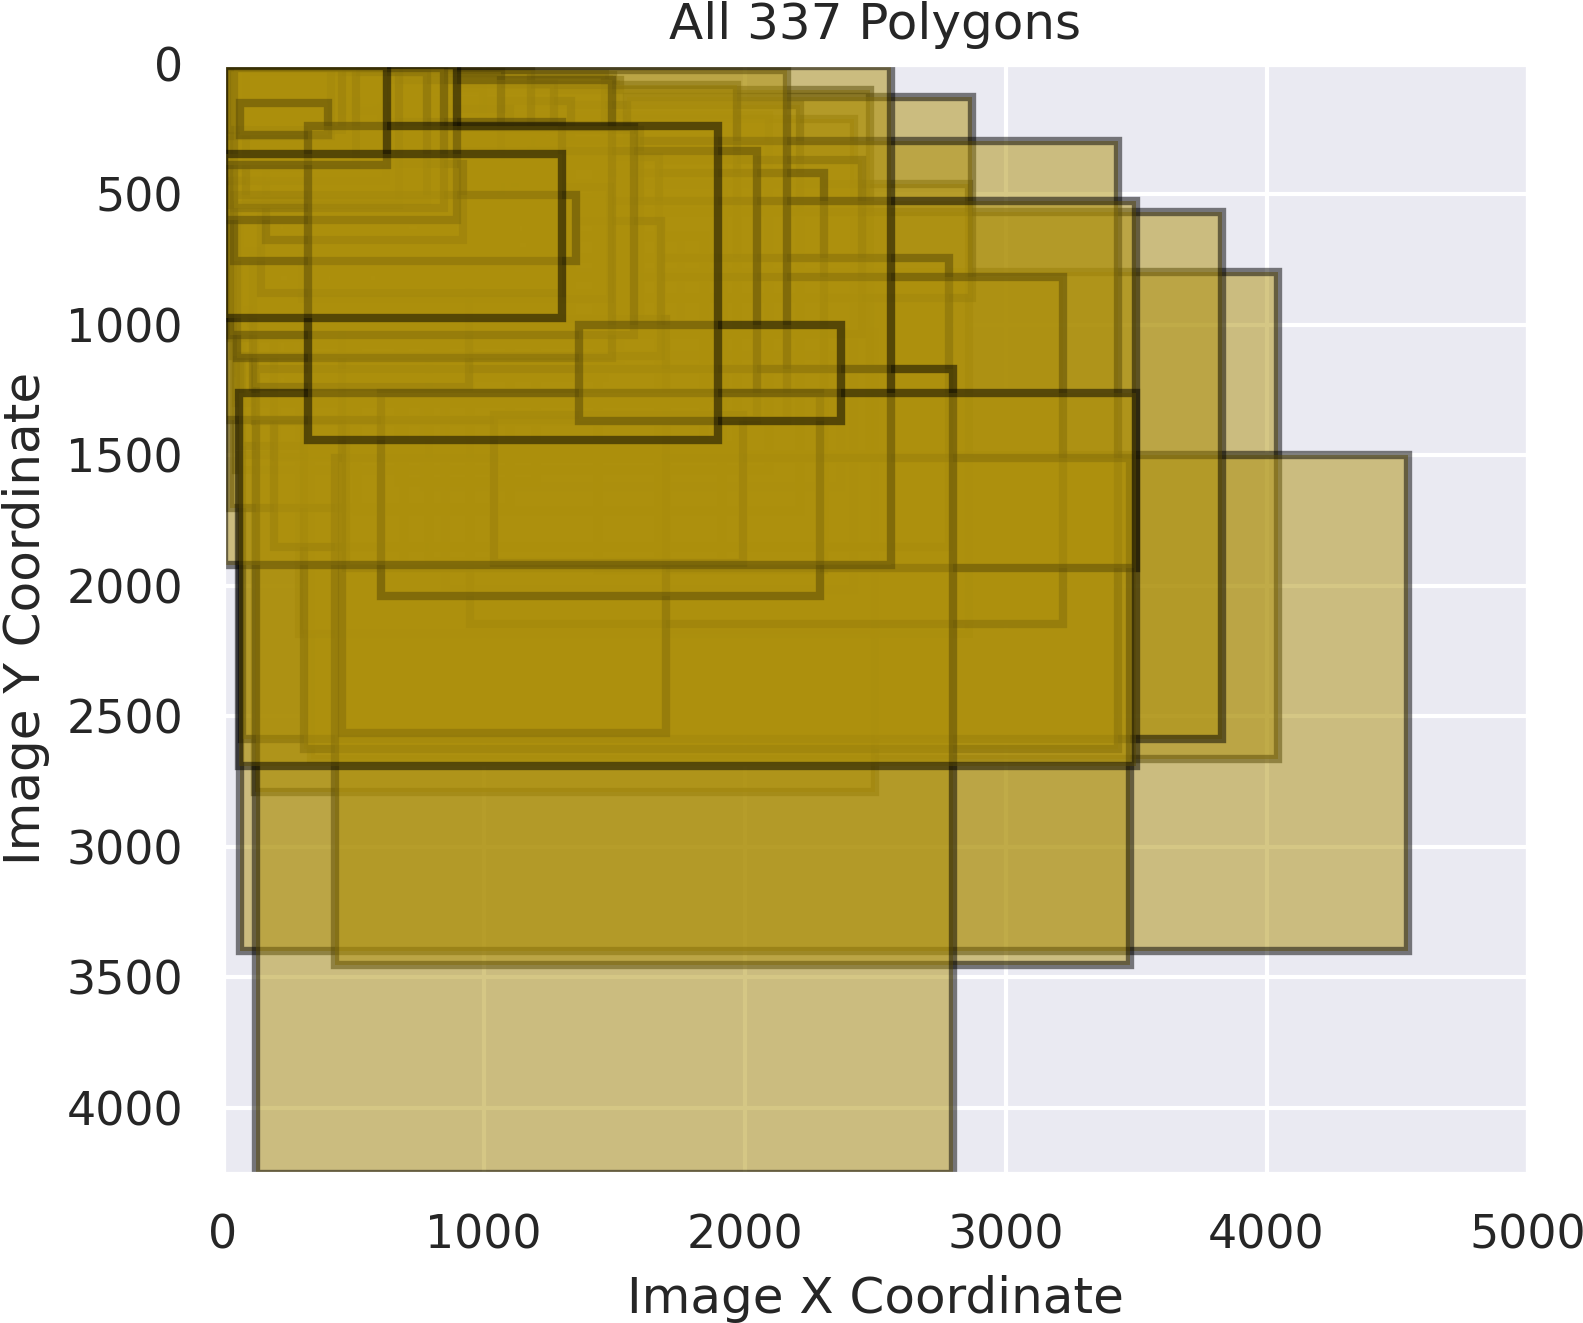
\includegraphics[width=0.4\textwidth]{figures/all_polygons.png}
\caption[]{
    All polygon annotations drawn in a single plot with 0.8 opacity to
    demonstrate the distribution in annotation location, shape, and size with
    respect to image coordinates. Annotations drawn with AI
    assistance tend to have more curved boundaries than manually drawn ones
    (several examples of manual annotations with more jagged boundaries can be
    seen in the top left).
}
\label{fig:AllPolygons}
\end{figure}

\begin{figure}[ht]
\centering
\includegraphics[width=0.4\textwidth]{figures/images_timeofday_distribution.png}
\caption[]{
    Scatterplot of the time-of-year vs time-of-day each image was taken. On the
    x-axis 0 is January 1st. On the y-axis 0 is midnight. For images with
    geolocation and timestamp (assuming the timezone is local or given and
    correct) we also estimate the amount of daylight as indicated by the color
    of each dot. While the majority of the images are taken in daylight, there
    are a sizable number of nighttime images.
}
\label{fig:TimeOfDayDistribution}
\end{figure}

\begin{figure}[ht]
\centering
\includegraphics[width=0.4\textwidth]{figures/spectra.png}
\caption[]{
    The "spectra" or histogram of the pixel intensities in the dataset. 
    The dataset rgb  mean/std is $[117, 124, 100], [61, 59, 63]$.
    % (for reference the imagenet mean/std is $[124, 116, 104], [58, 57, 57]$).
}
\label{fig:spectra}
\end{figure}


\begin{figure}[ht]
\centering
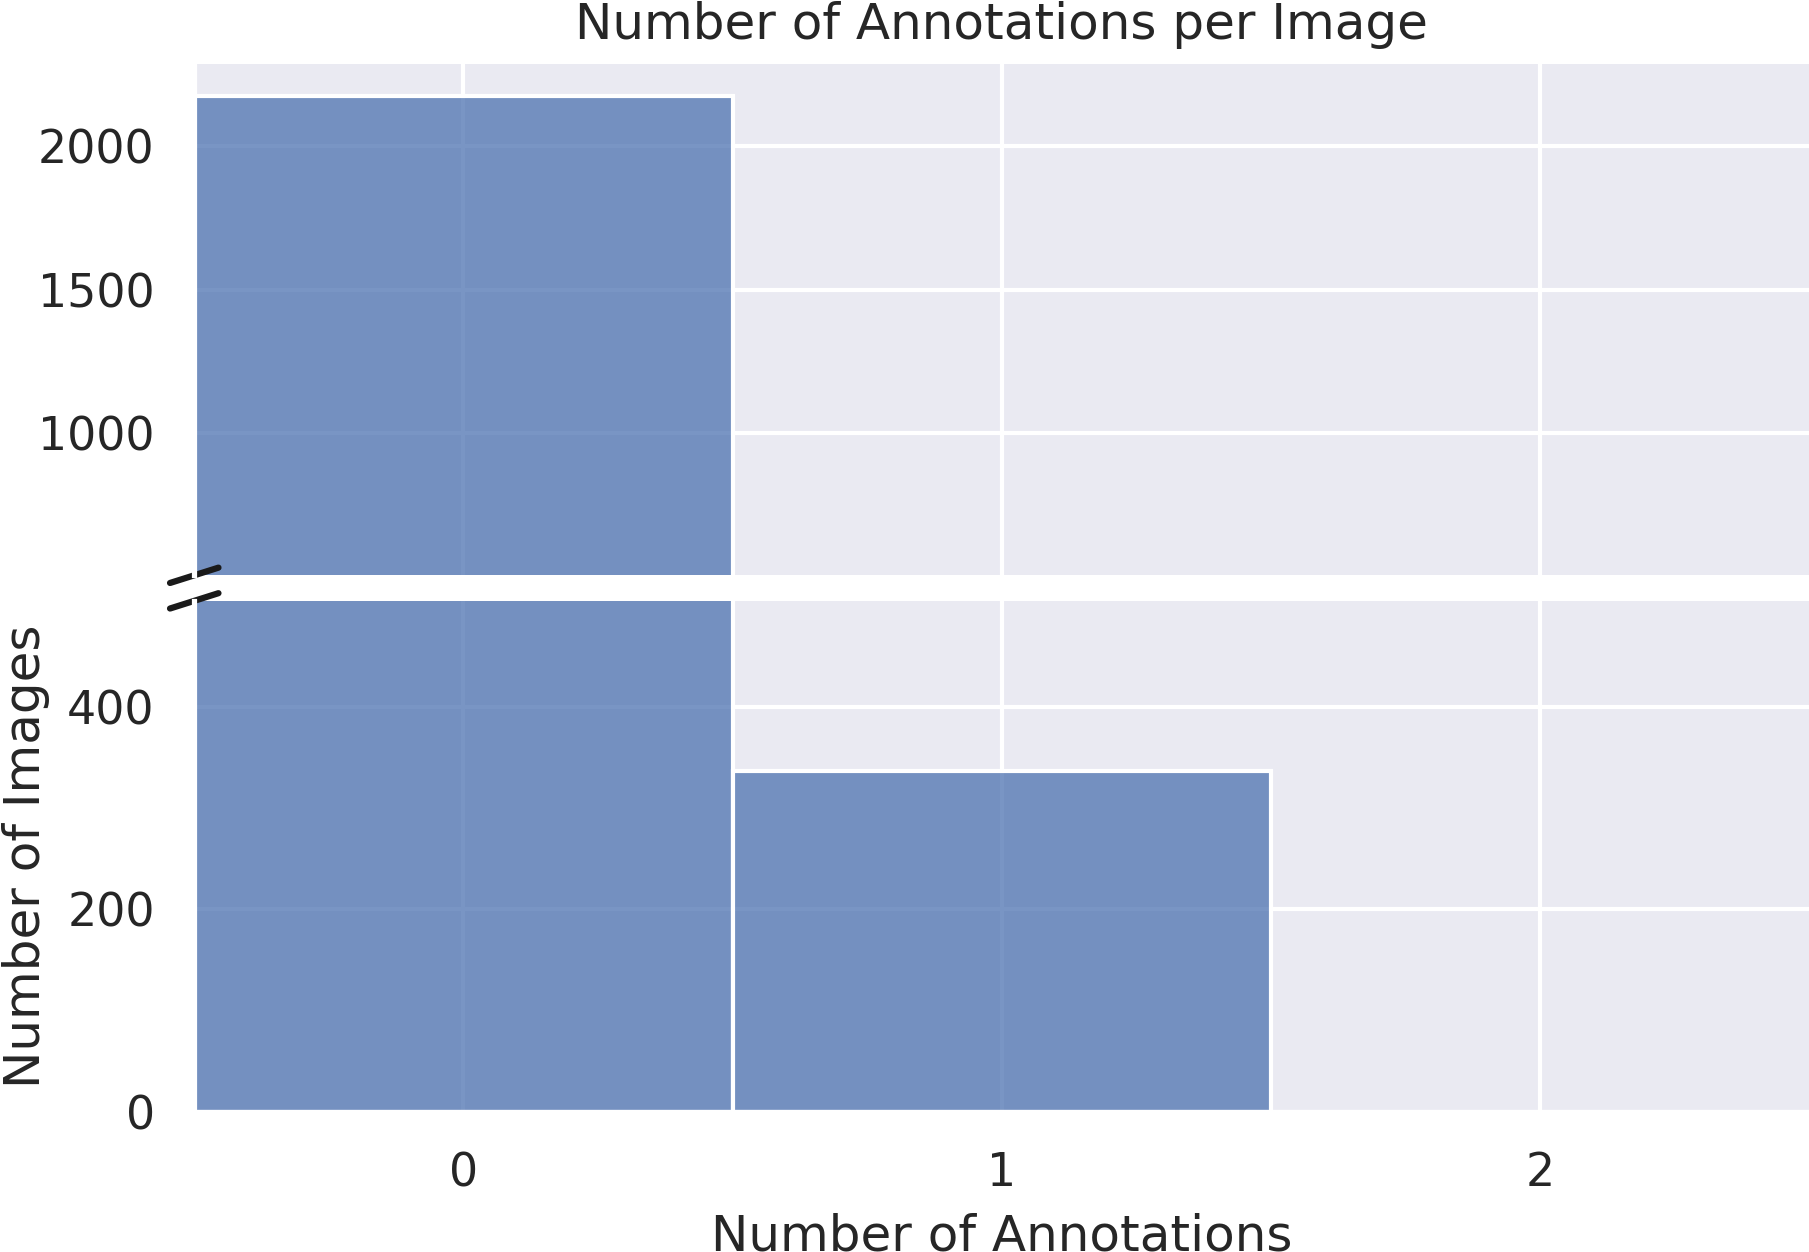
\includegraphics[width=0.4\textwidth]{figures/anns_per_image_histogram_splity.png}
\caption[]{
    Histogram of the number of annotations per image. 
    Only 35\% (2,346) of the images contain annotations, the other 65\% (4,302)
    are known not to contain poop. Of these 4,302 about half of them were taken
    directly after the poop was picked up, and the other half are pictures of a
    nearby location.
}
\label{fig:AnnotsPerImage}
\end{figure}


\subsection{Dataset Stats and Analysis}

% Number of images, annotations, and other stats.
As of 2024-07-03, the primary (i.e. training and validation) dataset contains
6648 images and 4386 annotations and has spanned 4 years. Data was captured
over 4 years at a mostly uniformly rate.  Most data is localized to parks and
sidewalks in a small city.  Weather conditions varied between snowy, sunny,
rainy.  The distribution of seasons, time-of-day, daylight, and capture rate is
illustrated in \Cref{fig:TimeOfDayDistribution}.

The dataset images are provided in full resolution and have not been resampled.
Almost all images were captured using the same phone-camera and have a
width/height of 4,032 $\times$ 3,024 (which could be rotated based on EXIF data) with 6
being 4008  $\times$ 5344 and one being 7,68 $\times$ 1,024. Images are stored as 8-bit JPEGs
with RGB channels, and most also contain overviews (i.e.  an image pyramid),
which makes loading a downscaled versions very fast.  The distribution of image
pixel intensities is shown in \Cref{fig:spectra}.


Due to the "B/A/N"-protocol, roughly 1/3 of the dataset has annotations due to
the other 2/3 of the images being taken in a way where the object of interest
was removed from the scene. Thus, most images have no annotations. The next
most frequent number of annotations is one, but images do often contain
multiple annotations.
There can be for several reasons for this:
    1) a single poop broke into multiple disjoint parts (the exact criteria for this is sometimes ambiguous), 
    2) two dogs pooped nearby each other. 
    3) one or more dogs has pooped in the same area over some period of
       time (some cases can be difficult to determine if it is poop or dirt).
The number of annotations per images is illustrated in
\Cref{fig:AnnotsPerImage}.

\subsection{Dataset Splits}

Data from 2021, 2022, 2023 are in the training set. Data from 2020 is used for
validation. Data from 2024 is split between training and validation. On the $n$th
day of the year, images are in the validation set if $n \% 3 == 0$ else they
are in the training set.

Specifically, in this paper our training dataset has 5747 images and can be
identified by a suffix of 1e73d54f, which is the prefix of a hash of its
contents.  The validation set contains 691 images and has a suffix of 99b22ad0.
The test set has a suffix of d8988f8c and consists of the 30 contributor images
that have at least one annotation.

\section{Models}

Our second contribution is an evaluation of several trained models to serve as
a baseline.  We use the training, prediction, and evaluation system of
\cite{Greenwell_2024_WACV, crall_geowatch_2024}, which uses polygon annotations
to train a pixelwise binary segmentation model.

In all experiments, we use half-resolution images, which means most images have
an effective width/height of 2,016 $\times$ 1,512. The samples given to the
network use a spatial widow size of 416 $\times$ 416, which means that multiple
windows are needed to predict on entire images. When we predict we use a window
overlap of 0.3 with feathered stitching is used to prevent boundary artifacts. 

Due to the imbalance of positive/negative (i.e. a positive is any patch that
contains an annotation, and a negative contains no annotations) in the dataset
we used a balanced sampling strategy.  Each "epoch" consisted of randomly
sampling 32,768 patches from the dataset with replacement.  The sampling was
balanced so the number of positives and negatives were roughly equal. In total
each network trained for 163,840 gradient steps. For data augmentation we use
random crops and flips.

The baseline architecture is a variant
\cite{bertasius2021space,Greenwell_2024_WACV} of a vision-transformer
\cite{dosovitskiy_image_2021}. The model has a 12 layer encoder backbone with
384 channels, and 8 attention heads. 
The segmentation head is a 4 layer MLP using encoder features.
The model has 25,543,369 parameters and a size of 114.19 MB on disk.
At predict time the model uses 1.961GB of GPU RAM.

Loss is computed pixelwise using FocalLoss \cite{ross2017focal} with a small
downweighting of pixels towards the edge of the window.  The optimizer is
AdamW, and we vary learning rate, weight decay, and perturb-scale (note: weight
decay combined with a non-zero perterb scale implements the shrink perturb
trick: \cite{ash_warm_starting_2020}).  We use a OneCycle learning rate
scheduler with a cosine annealing strategy and starting fraction of 0.3.  Our
effective batch size is 24 with a real batch size of 2 and 12 accumulate
gradient steps. At train time this consumes ~20GB of GPU RAM.


\subsection{Model Experiments}

In order to find a strong baseline we evaluated 35 different hyperparamter
training runs over different input resolutions, window sizes, model depth, and
other parameters in a somewhat ad-hoc manner. Taking the best hyperparameters
from that search, we perform a sweep over 7 combinations of learning rate,
weight decay, and perterb scale (i.e. shrink and perterb
\cite{ash_warm_starting_2020}). Scripts to reproduce these experiments as well
as a log of the ad-hoc experiments are in the code repo.
Models are also distributed with information about how they were trained.
%using stochastic engineer descent.


\begin{figure}[ht]
\centering

\includegraphics[width=0.4\textwidth]{figures/macro_results_resolved_params.heatmap_pred_fit.trainer.default_root_dir_metrics.heatmap_eval.salient_AP_vs_metrics.heatmap_eval.salient_AUC_PLT02_scatter_nolegend.png}

(a) AP and AUC of 35 checkpoints.

\includegraphics[width=0.4\textwidth]{figures/macro_results_resolved_params.heatmap_pred_fit.trainer.default_root_dir_metrics.heatmap_eval.salient_AP_PLT04_box.png}

(b) AP of 35 checkpoints.

\caption[]{
    (a) A scatterplot showing pixelwise AP and AUC for the top 5 checkpoints
    evaluated on the validation set. Points of the same color represent
    checkpoints from the same training run using identical hyperparameters.
    (b) The range of AP values across the top 5 checkpoints evaluated on the
    validation set. \Cref{tab:parameters_and_results} provides additional
    details on hyperparameters and maximum AP per run.
    %(a) A scatterplot of the pixelwise AP and AUC of the top-5 checkpoints evaluated on the validation set.
    %For each training run we ran evaluation on a subset of checkpoints that
    %achieved low validation loss.
    %Points with the same color represent checkpoints from the same training run
    %with with the same hyperparameters.
    %(b) The range of AP values over the top-5 checkpoints evaluated on the validation set.
    %\Cref{tab:parameters_and_results} provides more details about
    %hyperparameters and the maximum AP per run.
}
\label{fig:apauc_scatter}
\end{figure}

\begin{table*}[t]
\centering


\begin{tabular}{llllllll}
\toprule
            \multicolumn{4}{l}{} & \multicolumn{2}{c}{validation} & \multicolumn{2}{c}{test} \\
config name &   lr & weight\_decay & perterb\_scale & AP & AUC & AP & AUC \\
\midrule
        \textcolor[HTML]{623682}{D05} & 1e-4 &         1e-6 &          3e-6 &     \textbf{0.8325} &      \textbf{0.9927} &     0.5051 &      0.9125 \\
        \textcolor[HTML]{87b787}{D04} & 1e-4 &         1e-7 &          3e-7 &     0.8225 &      0.9795 &     0.4346 &      0.8576 \\
        \textcolor[HTML]{df8020}{D03} & 1e-4 &         1e-5 &          3e-7 &     0.8203 &      0.9679 &     0.4652 &      0.7965 \\
        \textcolor[HTML]{207fdf}{D02} & 1e-4 &         1e-6 &          3e-7 &     0.8159 &      0.9872 &     \textbf{0.5167} &      \textbf{0.9252} \\
        \textcolor[HTML]{20df20}{D00} & 3e-4 &         3e-6 &          9e-7 &     0.8107 &      0.9685 &     0.4210 &      0.7766 \\
        \textcolor[HTML]{df20df}{D01} & 1e-3 &         1e-5 &          3e-6 &     0.7665 &      0.9899 &     0.4607 &      0.9062 \\
        \textcolor[HTML]{b00403}{D06} & 1e-4 &         1e-6 &          3e-8 &     0.7458 &      0.9663 &     0.4137 &      0.8157 \\
\bottomrule
\end{tabular}
\caption{
    Scores for the best top model on the validation set for each of the 7 hyperparameter configurations. 
    These correspond to the maximum AP of each run in \Cref{fig:apauc_scatter}.
    The first column (config name) provides the code for a particular training run used in the score scatter and box plots.
    The next three columns correspond to the value of the varied hyperparameters that run.
    Then the AP and AUC scores on the validation set are given. The final two
    columns are the AP and AUC scores on the test set for these same
    validation-maximizing models models. (The top AP score on the test set was
    0.65, but it did not correspond to one of these validation runs used to
    select models).
    Qualitative examples on the test, validation, and training set are given in
    \cref{fig:test_heatmaps_with_best_vali_model} all on the top-scoring
    validation model listed here.
}
\label{tab:parameters_and_results}
\end{table*}

\begin{comment}
    SeeAlso:
    ~/code/shitspotter/experiments/run_pixel_eval_pipeline.sh
    python ~/code/shitspotter/dev/poc/estimate_train_resources.py
\end{comment}

Specifically, for each of the 7 hyperparameters we train the models for 163,840
optimizer steps using a batch size of 24. We consider an "epoch" as 1,365
steps, at which point we save a checkpoint, evaluate validation loss, and
adjust learning rates. To keep disk usage reasonable, we only keep at least the
top 5 lowest validation-loss checkpoints (training crashes and restarts
sometimes left more checkpoints on disk, and these were also included in our
evaluation).

Given these top-checkpoints on disk, we predict heatmaps for each image in the
validation set. Given a threshold we perform binary classification on each
pixel (poop-vs-background).  Then we rasterize the truth polygons at the same
prediction resolution (1/2 the resolution of full images). These corresponding
truth and predicted pixels are accumulated into a confusion matrix and 
standard measures precision, recall, F1, etc... \cite{powers_evaluation_2011} 
are computed for the specific threshold. By sweeping a threshold we can
compute the average precision (AP) and the area under the ROC curve that plots
recall to false positive rate (AUC). We compute all metrics with scikit-learn
\cite{scikit-learn}. Due to the high number of true negative pixels we prefer
the AP as the primary measure of model quality.

%\subsubsection{Results}

For each of the 7 training runs, we plot the AP and AUC of the top 5
AP-maximizing results. We also make plot a box and whisker for these top 5
results, which also serves to assign a color and label to each training run.
These are shown in \Cref{fig:apauc_scatter}. Details about the top model for
each run along with relevant hyperparameters for the training run are given in
\Cref{tab:parameters_and_results}. This table also shows the results on the
small --- but held out --- test set for the top model.

These results show strong performance on the validation set with a maximum AP
of $0.83$. However, while the test AP for this model is good, it is much lower
with an AP of $0.5051$. To investigate why this is we turn towards examples.

Qualitative results for the test, validation, and training set are shown in
\cref{fig:test_heatmaps_with_best_vali_model}. These examples illustrate
success and failure cases. The test and validation set both show clear
responses to the objects of interest. However, the test set often fails on
close up and partially-deteriorated poops. This hints at a bias in the dataset
towards "fresh" poops taken from some distance.

Notably the much larger training set also contains errors. This indicates that
there is still more information that can be extracted from this dataset,
perhaps with hard mining techniques. There are clear difficult cases in certain
sticks, leafs, and dark areas on snow. We note that while compiling these
results we discovered 14 cases where an object failed to be annotated, and it
is likely that more are missed, but we do believe these cases to be rare.

% If we found 14 cases, and we checked 1000 cases, and there is a 20%
% probability we miss a case, how many more missed cases do we expect to have?
% Chat GPU says
%To calculate the expected number of missed cases, you can use the following approach:

%Identify the expected number of true cases:

%If 14 cases were found, and there's a 20% probability of missing each case, you can estimate the total number of cases as:
%Total cases = 14 1 − 0.2 = 14 0.8 = 17.5
%Total cases= 1−0.2 14
%​
% = 0.8 14 ​ =17.5
%Calculate the number of missed cases:

%The expected number of missed cases would be:
%Missed cases = 17.5 − 14 = 3.5 Missed cases=17.5−14=3.5
%So, you would expect approximately 3 to 4 more missed cases.

Even though focal loss was used, the current learning curriculum is likely
under weighting smaller distant objects. Our pixelwise evaluation metric is
biased against it, which is a current limitation.

\begin{figure*}[ht]
\centering
\includegraphics[width=1.0\textwidth]{figures/test_heatmaps_with_best_vali_model}%
\hfill
(a) test set
\includegraphics[width=1.0\textwidth]{figures/vali_heatmaps_with_best_vali_model.jpg}%
\hfill
(b) validation set
\includegraphics[width=1.0\textwidth]{figures/train_heatmaps_with_best_vali_model.jpg}%
\hfill
(c) training set
\caption[]{
    Qualitative results using the highest scoring model on the validation set
    on a selection of images from (a) the test test, (b) the validation set and
    (c) the training set.
    Success cases are on the left, and failures increase towards the right.
    %
    In each figure, the top rows shows true positive pixels in white, false
    positive pixels in red, false negative pixels in teal, and true negative
    pixels in black.  For visualization purposes, the threshold to binarize the
    prediction is chosen to maximize the F1 for each image, thus the top row is
    in some sense the best possible classification of the heatmap, which is
    shown in the middle row. The final row is the input image.
    %
    Most images in the (small, 30 image) test set are qualitatively good.
    Failure cases are limited to close up images of older sometimes
    partially-deteriorated poops.

    These examples were manually selected and ordered by hand. (could recompute
    the order based on some measure).
}
\label{fig:test_heatmaps_with_best_vali_model}
\end{figure*}


\subsubsection{Resource Usage}


\begin{table}[t]
    \centering
\begin{tabular}{llllr}
\toprule
        node & resource &           total &            mean &  num \\
\midrule
eval  & time            & 07:52:02 &  00:13:29 &   35 \\
\midrule
pred  & time            & 04:23:34 &  00:07:32 &   35 \\
pred  & electricity     & 3.17 kwh &     0.091 kwh&   35 \\
pred  & emissions       & 0.67 \cotwo kg &     0.02 \cotwo kg &   35 \\
\midrule
train$^{*}$ &   time    & 39.2 days  & 5.60 days&   7 \\
train$^{*}$ &   electricity  & 329.4 kwh &     47.1 kwh &   7 \\
train$^{*}$ &   emissions & 69.2 \cotwo kg &     9.9 \cotwo kg &   7 \\
\bottomrule
\end{tabular}
(a) presented experiment resources
\begin{tabular}{llllr}
\toprule
        node & resource &           total &            mean &  num \\
\midrule
% Note: for presentation simplicity, we are rewriting the following row
% so num agrees with other rows. The reason the original value had an
% additional number is because of rerun of one evaluation with different
% parameters.
% eval & time & 4 days 14:18:23 & 00:20:07 &  330 \\
eval & time & 4 days 14:18:23 & 00:20:07 &  329 \\
\midrule
pred & time & 6 days 06:52:11 & 00:27:31 &  329 \\
pred & electricity &       85.31 kWh &        0.26 kWh &  329 \\
pred & emissions &       17.95 \cotwo kg &        0.05 \cotwo kg &  329 \\
\midrule
train$^{*}$ &   time &        158.9 days &         3.75 days &   42 \\
train$^{*}$ & electricity &   1335.14 kWh &       31.79 kWh &   42 \\
train$^{*}$ & emissions &   280.4 \cotwo kg &        6.7 \cotwo kg &   42 \\
\bottomrule
\end{tabular}
(b) all experiment resources
\label{tab:resources}
\caption[]{
Resources used for training, prediction, and evaluation are detailed in two tables:
(a) resources for the presented evaluations, and (b) resources for prior hyperparameter tuning.
The left column identifies the pipeline stage:
"train" for training, "pred" for heatmap prediction, and "eval" for pixelwise heatmap evaluation.
The second column lists the resource type: time (in days or hours), electricity (in kWh), or emissions (in
  kg of \cotwo{}).
The following columns show the total and average consumptions, and the final column indicates the
  frequency of each stage (e.g., across different hyperparameters).
Train rows marked with an asterisk (*) are based on indirect measurements.
%Time estimates are based on timestamps from checkpoint files.
%Energy consumption assumes a constant 350W power draw for a 3090 GPU.
%Emissions are calculated using a conversion ratio of 0.21 kg \cotwo{} / kWh.
%Resources consumed to train, predict and evaluate models.
%These numbers are broken into two tables: (a) resources used in the presented
%evaluations and (b) resources used in hyperparameter tuning beforehand.
%The leftmost column indicate the stage of the pipeline. This is "train" for
%training, "pred" for heatmap prediction, and "eval" for pixelwise heatmap
%evaluation.
%The second column indicates the resource: time is measured in days or hours.
%electricity is measured in kilowatt hours (kwh), and emissions are measured in
%kilograms of \cotwo{} emitted by the electricity consumption.
%The next two columns give the total and average quantity of the consumed
%resource, and the final column indicates the number of times a particular stage
%was performed (e.g. over different hyperparameters).
%Note: that training numbers marked with an $*$ to indicate they are based on
%estimates and not direct measurements.
%To indirectly measure time we used timestamps on on checkpoint and log files.
%For energy we assumed constant use of the maximum 350W power draw of
%a 3090 GPU. For emissions we use a 0.21 conversion ratio to convert kilowatt
%hours to kilograms of carbon emissions.
%Note: this table does not include training time, which was not measured
%directly at the time. Our stated train time estimates are based on.
}
\end{table}

All models were trained on a single machine with an 11900k CPU and a 3090 GPU.
At predict time, using 1 background worker, our models processed 416 $\times$
416 patches at a rate of 20.93Hz with 94\% GPU utilization.

We measure the predict and evaluation time resource usage using CodeCarbon
\cite{lacoste2019codecarbon}.
The resource utilization for the presented 7 training experiments and the 42
total training experiments are reported in
% \Cref{tab:resources}. % wtf
Table \ref{tab:resources}.
% See: ./scripts/estimate_training_resources.py
Direct measurement of resource usage during training is still under
development. However, we estimate the duration of each training run using
indirect methods. Electricity consumption is approximated by assuming a maximum
power draw of 350W for a 3090 GPU. Emissions are calculated using a conversion
ratio of 0.21 from kilowatt hours to kilograms of \cotwo{}.

%However, the experiments presented here were not the only ones performed in
%determining the hyperparameters we held constant here. 
%The path to the presented experiments involved trying over 42 training run with
%a wider variation of parameters. 


\section{Open Data Distribution}

% BitTorrent can be vulnerable to MITM:
% https://www.reddit.com/r/technology/comments/1dpinuw/south_korean_telecom_company_attacks_torrent/

Our third contribution is an exploration and observational study of distributed
and centralized data distribution methods. 

%Advantages of content addressability:
%* reproducibility 

The well-documented reproducibility "crisis" in science has raised significant
concerns across various disciplines \cite{baker_reproducibility_2016}. Ideally,
all scientific research should be independently reproducible; however, even in
computer science, reproducibility success rates are reported to be around 60\%.
Although this is higher than in other scientific fields, there is still room
for improvement \cite{NEURIPS2019_c429429b, collberg2016repeatability,
desai_what_2024}.

The challenge lies in the fact that designing and documenting an experiment
sufficiently for reproducibility requires substantial effort and is prone to
error. We suggest that reducing the friction in accessing the necessary data
could improve these success rates. Specifically, this involves codifying data
download and preparation processes. Datasets that are available via distributed
and content-addressable are particularly advantageous, as they can guarantee
the integrity of the data prevent the issue of dead URLs.

Centralized data distribution has many advantages. It is fast and has low
traffic overhead. However, it is prone to failure.  
Cloud storage for a modest amount of data can be expensive.

In contrast, Decentralized methods can allow information to persist so long as
at least 1 person has the data.

However, there are certain drawbacks of distributed dataset distribution to
consider. One significant limitation is the potentially substantial connection
time required to link with peers, particularly when the data lacks a sufficient
number of "seeders". Furthermore there needs to be a mechanism to connect to
peers that can share the data.

Despite the disadvantages, distributed methods can guarantee accessibility in a
way that centralized mechanisms fundamentally cannot.  It is for this reason we
are motivated to investigate distributed methods.

The well known BitTorrent \cite{cohen_bittorrent_2017} data sharing system
originally relied on centralized trackers and databases of torrent files to
connect peers.  While trackers and torrent files are still prominent, modern
torrents can be published to a distributed hash table (DHT) using the Kademlia
algorithm \cite{maymounkov_kademlia_2002}. This makes it an strong candidate
for a distributed distribution mechanism. 

Another candidate system is a newer similar tool called IPFS (InterPlanetary
File System) \cite{benet_ipfs_2014, bieri_overview_2021}. To quote the authors:
"IPFS could be seen as a single BitTorrent swarm, exchanging objects within one
Git repository". All data down to the block level is content addressable and
stored in a Merkle DAG, which can simply data versioning compared to using a
torrent.

%IPFS vs BitTorrent:

A comparison of IPFS and BitTorrent on the protocol level is beyond the scope
of this paper. A high level overview of details is provided in
\cite{zebedee_comparing_2023}.  Both IPFS and BitTorrent are both effectively
content addressable, which makes them both appropriate for our use case. We
care about accessing the data quickly in order to use it.  Thus, our comparison
is going to focus on download-time measurements.
%Both of which have the ability to use the Kademlia - distributed hash table (DHT) \cite{maymounkov_kademlia_2002}.
%IPFS always uses its DHT, where as BitTorrent the Kademlia-based Mainline
%Tracker can be disabled in favor of 3rd party trackers.
% Overview and comparison of protocols via github gist:
% https://gist.github.com/liamzebedee/224494052fb6037d07a4293ceca9d6e7
% https://gist.github.com/liamzebedee/4be7d3a551c6cddb24a279c4621db74c
%[Steiner, En-Najjary, Biersack 2022]
% See Also:
% Long Term Study of Peer Behavior in the KAD DHT
% https://git.gnunet.org/bibliography.git/plain/docs/Long_Term_Study_of_Peer_Behavior_in_the_kad_DHT.pdf
% We have been crawling the entire KAD network once a day for more than a year to track end-users with static
% IP addresses, which allows us to estimate end-user lifetime and the fraction of end-users changing their KAD ID.

%Both BitTorrent (starting with the v2 protocol introduced in 2017 \cite{cohen_bittorrent_2017}) and IPFS have the capability to recognize when two torrents or content identifiers (CIDs) contain the same file. This enables seeders to provide files to downloaders of either torrent or CID, enhancing the availability and redundancy of the data.
%Both BitTorrent (as of 2017 in the v2 protocol \cite{cohen_bittorrent_2017})
%and IPFS can recognize that two torrents/CID include the same file and seeders
%can provide files to downloaders of the other.


%Additionally, storing data in the cloud can become prohibitively expensive,
%even for modest amounts of data. In contrast, decentralized methods allow
%information to persist as long as at least one individual retains the data.

%Discuss distributing the dataset via IPFS versus centralized distribution
%systems.
%Decentralized Method - IPFS and BitTorrent.
%Centralized Method - Girder


\subsection{Distribution Observational Study}

To assess the effectiveness of distributed distribution of datasets, we perform
an observational study. We attempt to download the dataset via each of the 3
primary distribution mechanisms, and measure the time it takes to complete.
For distributed methods, there wasn't a clear automated mechanism to measure
lag-time for connecting to peers, which was a significant issue in these tests.

As an example centralized distribution mechanism we use the Girder
\cite{girder_2024} data management platform.
For bittorrent we use the transmission-client \cite{transmission_2024}.
For IPFS we use the standard kubo implementation \cite{girder_2024}.
We also include direct "rsync" \cite{rsyncprojectrsync_2024} between machines as a baseline method.

A difference between the girder and decentralized methods is that the former
required that the data was packaged into separate zip files, which could
improve transfer efficiency due to fewer file boundaries.

In all tests, the source and destination machines are separated by about 30
kilometers with an average ping time of 48.480ms. For each test we create a
measurement log (included in supplemental materials) and record the start
time and end time of the transfer. We also include notes and command line
invocations.

The average durations between the start of the transfer command and its
completion are shown in \cite{tab:transfertime}.

\begin{table}[t]
\begin{tabular}{llllll}
\toprule
{} & count &   mean &    std &   min &    max \\
method        &       &        &        &       &        \\
\midrule
bittorrent & 5 & 8.36 & 5.16 & 2.21 & 14.39 \\
ipfs & 3 & 4.14 & 2.13 & 1.80 & 5.96 \\
rsync & 2 & 4.60 & 2.12 & 3.10 & 6.10 \\
girder & 3 & 1.24 & 0.16 & 1.05 & 1.33 \\
\bottomrule
\end{tabular}
\label{tab:transfertime}
\caption[]{
    Number of hours of transfer speeds of entire dataset averaged of n trials,
    noted in the "count" column. 
}
\end{table}


In addition to these measurements we have made several anecdotal observations
that are worth discussing.

\begin{itemize}
    \item IPFS via https using gateways does not always work well.
    \item IPFS usually works well if you use the CLI.
    \item IPFS is easier to update.
    \item IPFS does rehash every file, which induces an O(N) scalability constraint.

    \item BitTorrent and IPFS seem to both take awhile to establish connection
          to a peer when there are a small number of pinners/seeders.

          IPFS has a mechanism to directly connect to a peer, which seems to
          work fairly quickly, but not immediately.

          This issue is mitigated as the number of seeders/pinners grows.
          A test download of ImageNet LSVRC 2017 dataset from academic torrents
          almost immediately connected to 2 seeders.

    \item Centralized solutions depend on an organization providing a service,
          and that organization can choose to stop providing that service.
\end{itemize}

The specific version of the dataset used in this paper was snap-shotted on
2024-07-03 and has the IPFS content ID of:

\begin{lstlisting}[basicstyle=\normalsize]
bafybeiedwp2zvmdyb2c2axrcl455x
fbv2mgdbhgkc3dile4dftiimwth2y
\end{lstlisting}

The torrent is tracked on Academic Torrents \cite{academic_torrents_Cohen2014} and has a magnet URL of:

\begin{lstlisting}[basicstyle=\normalsize]
magnet:?xt=urn:btih:
ee8d2c87a39ea9bfe48bef7eb4ca12eb68852c49
\end{lstlisting}

% https://academictorrents.com/docs/about.html

% magnet:?xt=urn:btih:ee8d2c87a39ea9bfe48bef7eb4ca12eb68852c49&tr=https%3A%2F%2Facademictorrents.com%2Fannounce.php%3Fpasskey%3D9ffbb169f882f3be1330a48ea87416e7&tr=udp%3A%2F%2Ftracker.coppersurfer.tk%3A6969&tr=udp%3A%2F%2Ftracker.opentrackr.org%3A1337%2Fannounce



%-------------------------------------------------------------------------
\section{Related Work}


The ImageNet dataset \cite{ILSVRC15}.

The MSCOCO dataset \cite{lin_microsoft_2014}.

Object detection

Waste detection is an important problem but with relatively few open datasets.
%  https://paperswithcode.com/dataset/zerowaste
The ZeroWaste dataset \cite{bashkirova_zerowaste_2022} contains 1,800 segmented
video frames and 6000 unlabeled frames in a recycling facility.
% https://paperswithcode.com/dataset/taco
The TACO dataset \cite{proenca_taco_2020} is another "living" dataset
containing 1500 images with 4,784 annotations over 60 classes.
% TrashCan https://paperswithcode.com/dataset/trashcan
% Top Datasets on paperwith code
% https://paperswithcode.com/datasets?mod=images&task=semantic-segmentation&page=2


% Domestic Trash / Garbage Dataset
% Looks like the full dataset is behind a paywall
% https://paperswithcode.com/dataset/domestic-trash-garbage-dataset


% https://universe.roboflow.com/dataset-vmyna/poop-yxidr/dataset/1
% 102 train images, 22 validation images, 0 test images.
% human poop


While ours is the largest publicly available poop dataset that we are aware of,
it is not the first.
A dataset of 100 dog poop images was collected and used to train a FasterRCNN
model in 2019 but this dataset and model are not publicly available \cite{neeraj_madan_dog_2019}.
The MSHIT dataset \cite{mshit_2020} consists of 3.89GB of real images with fake
poop (e.g. plastic poop) in controlled environments.
The company iRobot has a dataset of annotated indoor poop images used to train
Roomba j7+ to avoid collisions, but as far as we are aware, this is not
available \cite{roomba_2021}.


IPFS and BitTorrent are the distributed distribution mechanism we consider, but there are others

% Very good overview and comparison of the protocols
% https://blog.mauve.moe/posts/protocol-comparisons
% https://distributed.press/
% hypercore - https://github.com/tradle/why-hypercore/blob/master/FAQ.md#how-is-hypercore-different-from-ipfs
% git,
% Secure Scuttlebut (SSB)

\section{Conclusion}

The ShitSpotter dataset is 42GB of images with polygon segmentations of dog
poop. 

We train and evaluate several baseline segmentation models, the best of which
achieves an AP/AUC of 0.8325 on the validation set and 0.5051 on the test set.

Our dataset is sufficient to train an object detection network to (level of
precision/recall).
Our experimental evaluation is limited by lack of model diversity, but it
serves as a baseline for future exploration.

We make data and models available over 3 distribution mechanisms: 
cloud storage, BitTorrent, and IPFS.

Decentralized methods are feasible methods of distribution, with strong
security but they can be slow.
IPFS is a promising solution for hosting scientific datasets, but does have pain points.
In contrast bittorrent can do X/Y/Z, but ...
Lastly centralized cloud storage can give the best speeds, but sacrifices some
security and can be less robust.

Directions for future research / development are:
1) Add lightweight object-level head and test object detection metrics.
2) Optimize model architectures for mobile devices.
3) Launch phone application.
4) Improve model / data distribution.


%%%%%%%%% REFERENCES
{\small
\bibliographystyle{ieee_fullname}
\bibliography{citations}
}
%\bibliographystyle{unsrtnat}
%\bibliography{references}  %%% Uncomment this line and comment out the ``thebibliography'' section below to use the external .bib file (using bibtex) .


\begin{comment}
    cd $HOME/code/shitspotter
    python -m shitspotter.cli.coco_annotation_stats $HOME/data/dvc-repos/shitspotter_dvc/data.kwcoco.json \
        --dst_fpath $HOME/code/shitspotter/coco_annot_stats/stats.json \
        --dst_dpath $HOME/code/shitspotter/coco_annot_stats

    SeeAlso:
    ~/code/shitspotter/experiments/run_pixel_eval_pipeline.sh
    ~/code/shitspotter/experiments/run_pixel_eval_on_test_pipeline.sh
    ~/code/shitspotter/experiments/run_pixel_eval_on_train_pipeline.sh

    python ~/code/shitspotter/dev/poc/estimate_train_resources.py

    See: ./localize_figures.sh


    Best Validation Model:
        /home/joncrall/data/dvc-repos/shitspotter_expt_dvc/training/toothbrush/joncrall/ShitSpotter/runs/shitspotter_scratch_20240618_noboxes_v7/lightning_logs/version_1/checkpoints/epoch=0089-step=122940-val_loss=0.019.ckpt.pt
        # Best Rank:  33.0 pyzvffmyjcrq
        Lives in /home/joncrall/data/dvc-repos/shitspotter_expt_dvc/_shitspotter_test_evals/eval/flat/heatmap_eval/heatmap_eval_id_0f613533/pxl_eval.json heatmap_eval           pyzvffmyjcrq    0.505110     0.912509
        

    Best Test Model:
        /home/joncrall/data/dvc-repos/shitspotter_expt_dvc/training/toothbrush/joncrall/ShitSpotter/runs/shitspotter_scratch_20240618_noboxes_v6/lightning_logs/version_0/checkpoints/epoch=0073-step=101084-val_loss=0.017.ckpt.pt
        is Rank 3 on the validation dataset.
    

    cd /home/joncrall/code/shitspotter/shitspotter_dvc
    geowatch spectra --src data.kwcoco.json --workers=16 --cache_dpath=_spectra_cache --dst spectra.png --bins 64 --valid_range=0:255
    cp spectra.png ~/code/shitspotter/papers/application-2024/figures/spectra.png

\end{comment}

\end{document}
